\section{TraceBound: Methodology and Implementation Details}
\subsection{Problem setting and interface}
Each example consists of a natural-language query $q$, a text-rich knowledge graph $G=(V,E)$, and a gold answer set $Y \subseteq V$. A retrieval agent returns an ordered list $\hat{Y}=(v_1,\ldots,v_k)$, which is evaluated with \hit{1}, \hit{5}, \recall{20}, and \mrr. The agent can call two graph tools: \emph{global search}, which retrieves candidate nodes from textual descriptors, and \emph{neighborhood exploration}, which expands a selected node through one-hop relations. The controller operates in an action-observation loop until it emits final answers or reaches a maximum interaction budget.

\subsection{The TraceBound intervention}
\tb adds profile conditioning and trace conditioning to this controller. The input remains the original query and graph; the output remains a ranked node list plus an execution trajectory. The intervention changes the controller context, not the task definition.

\paragraph{Query profile.}
Before the first tool call, \tb asks the controller to form a compact profile containing predicted answer type, important query facets, relation hints, and retrieval risks. The profile is not a user memory; it is a query-derived stand-in for the kind of compact state that a personalized retriever would eventually use. Its purpose is to test whether an explicit pre-retrieval state helps the controller decide how to search.

\paragraph{Trace hints.}
After each observation, \tb updates a trace state with counters for global calls, neighborhood calls, zero-result calls, repeated calls, step count, and remaining budget. The controller receives a short diagnostic hint only when the trace indicates a potential failure pattern, such as repeated identical calls or empty neighborhoods. The hint is intentionally constrained; it can recommend re-anchoring, relaxing a constraint, tightening type focus, or stopping, but it does not reveal labels or gold answers.

\paragraph{Instrumentation.}
Every trajectory is logged as a sequence of actions, observations, and counters. This lets us compute paired process metrics on the same examples used for ranking evaluation. The key design choice is separation - ranking metrics are computed only from final answer lists, while trace metrics are computed only from trajectories.

\begin{figure*}[t]
\centering
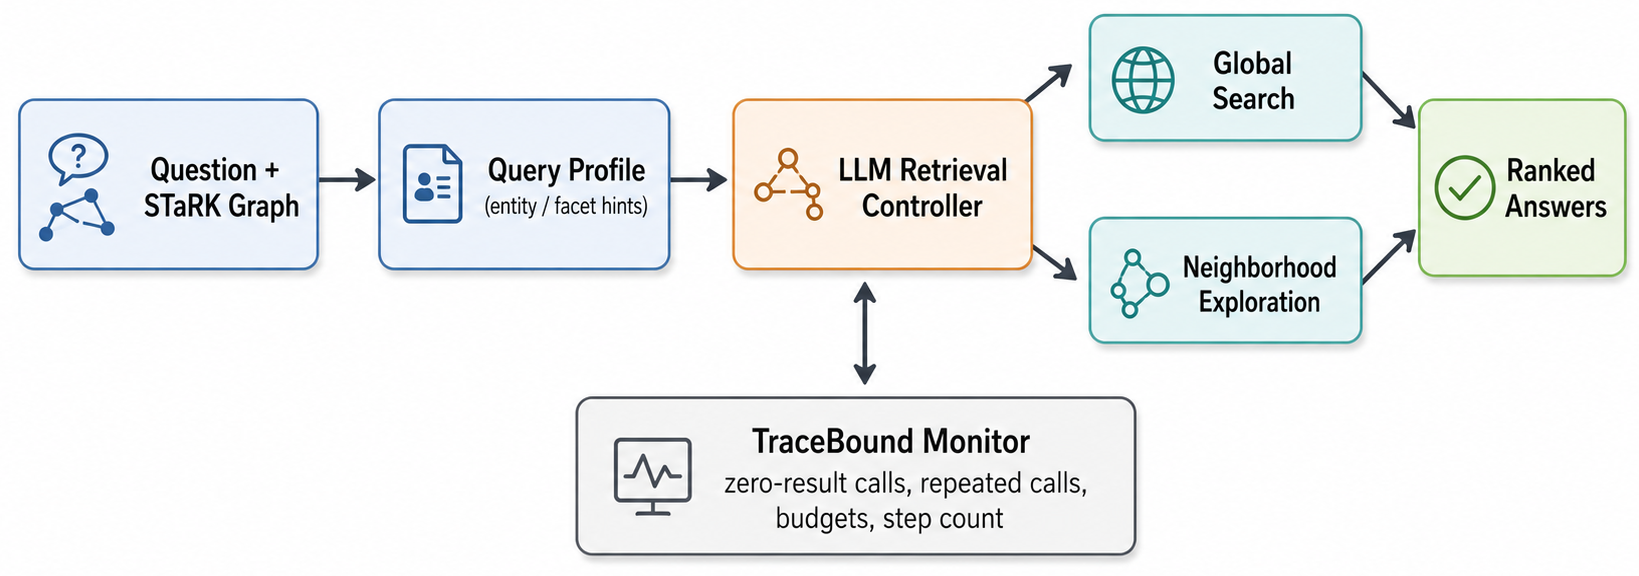
\includegraphics[width=\textwidth]{figures/tracebound_pipeline.png}
\caption{\textbf{TraceBound workflow.} The input query and graph are passed to an ARK-style controller. \tb adds a query-profile block before retrieval and a monitor that summarizes zero-result calls, repeated calls, budget use, and step count during retrieval. The graph tools and final ranking evaluator are unchanged. The ranked answers produce \hit{1}, \hit{5}, \recall{20}, and \mrr, while the monitor produces trace diagnostics used only for analysis.}
\label{fig:pipeline}
\end{figure*}

\subsection{Evaluated controller variants}
Table~\ref{tab:modes} defines the four variants. The unconditioned agent is the baseline: it receives the original query, tool descriptions, and prior observations, but no additional profile or trace hint. Profile-only and trace-only isolate the two ingredients. \tb combines both.

\begin{table}[t]
\centering
\caption{\textbf{Controller variants.} ``Profile'' means the controller receives a compact pre-retrieval query profile. ``Trace hint'' means the controller receives short observation-level feedback derived from trajectory counters. ``Logged diagnostics'' means the trajectory is converted into process metrics; these metrics are not used by the final ranking evaluator.}
\label{tab:modes}
\resizebox{\columnwidth}{!}{%
\begin{tabular}{lccc}
\toprule
Variant & Profile & Trace hint & Logged diagnostics \\
\midrule
Unconditioned agent & no & no & final-answer metrics \\
Profile-only agent & yes & no & profile metadata \\
Trace-only agent & no & yes & process counters \\
\tb agent & yes & yes & profile + process counters \\
\bottomrule
\end{tabular}}
\end{table}

\subsection{Algorithmic summary}
Given a query $q$, \tb first constructs a query profile $p(q)$. At step $t$, the controller observes the query, profile, previous observations, and current trace summary $s_t$. It chooses either global search, neighborhood exploration, or final-answer emission. After a tool call, the monitor updates $s_{t+1}$ by checking whether the result was empty, whether the call repeated an earlier call, how much budget remains, and whether enough candidates have been accumulated. The method is therefore not a new retriever index; it is a controller-side protocol for profile-conditioned action selection and trace-conditioned diagnostics.

\subsection{Design invariants}
A diagnostic intervention is only useful if it does not move the evaluation target. We therefore preserve five invariants. Table~\ref{tab:invariants} summarizes what is fixed and what is changed. The graph corpus, gold labels, retrieval metrics, and tool semantics remain fixed. The only manipulated object is the controller context and the logging attached to each action. This lets us attribute changes in ranking to the behavior of the adaptive policy rather than to a different retriever, different corpus, or different evaluator.

\subsection{What the trace can and cannot do}
The trace hint is not an oracle. It does not know whether a retrieved node is correct, and it does not inspect the gold set. It only summarizes observable symptoms. For example, if the controller repeats a global search with nearly identical arguments, the hint can recommend changing the anchor or stopping repeated exploration. If a neighborhood call returns no candidates, the hint can recommend relaxing the relation/type constraint or returning to global search. This keeps \tb close to deployment settings where a retrieval system can observe its own trajectory but cannot observe the correct answer during inference.

\subsection{State representation and action view}
The protocol can be written as a small partially observed control problem. At step $t$, the controller has a hidden retrieval belief induced by the prompt and an explicit trace state
\[
  s_t = (g_t, n_t, z_t, r_t, b_t, c_t),
\]
where $g_t$ counts global searches, $n_t$ counts neighborhood explorations, $z_t$ counts zero-result calls, $r_t$ counts repeated calls, $b_t$ is remaining budget, and $c_t$ summarizes the current candidate set. The controller chooses an action $a_t \in \{\textsc{Search},\textsc{Explore},\textsc{Answer}\}$. \tb changes the textual representation of $s_t$ exposed to the controller, while the evaluator observes only the final $\textsc{Answer}$ action. This view is useful because it makes clear why static prompts are limited: the important object is the conditional distribution over actions, not the mere presence of a trace string.


